\chapter{Resolução dos três problemas de programação}
\label{chap:fundamentacao-teorica}

\section{Problema 1}
%\label{sec:dmst}

O problema descrevia a situação de um professor que precisava distribuir pontos extras entre seus alunos de acordo com o número do aluno sorteado na lista, em ordem alfabética, de chamada, essa questão pedia que fosse criado um programa em que as primeiras entradas eram o número de pessoas na lista e o número sorteado e o programa deveria retornar o nome da pessoa sorteada. A \autoref{fig:questao 1} apresenta a submissão no site Beecrowd do codigo.


\begin{lstlisting}[language=Java, caption={Código de implementação do algoritmo de implementação do problema 1}, label={lst:codigo-problema1}]
import java.util.*;

public class Main {
    public static void main(String[] args) {
        Scanner scanner = new Scanner(System.in);
        
        int N = scanner.nextInt();
        int K = scanner.nextInt();
        scanner.nextLine(); 


        List<String> alunos = new ArrayList<>();

        for (int i = 0; i < N; i++) {
            alunos.add(scanner.nextLine());
        }

        Collections.sort(alunos);


        System.out.println(alunos.get(K - 1));

        scanner.close();
    }
}
\end{lstlisting}

\begin{figure}
	\centering
	\caption{Submissão da questão 1.}
	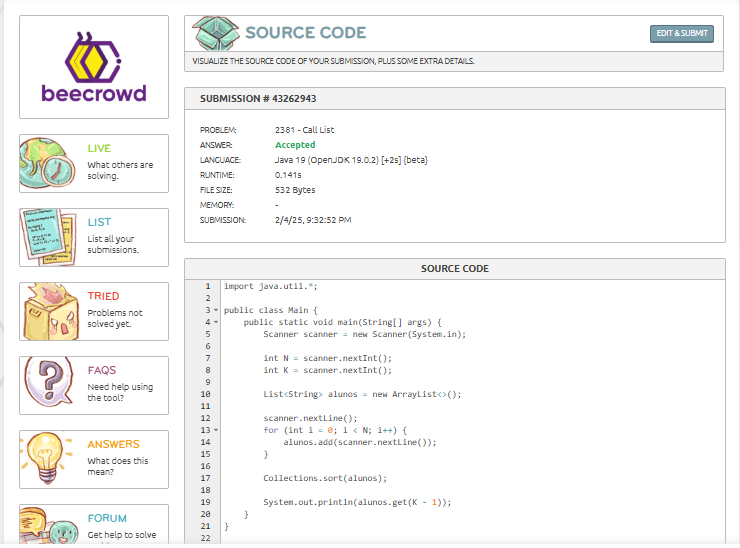
\includegraphics[width=0.7\textwidth]{figuras/questao 1.png}
	}
	\label{fig:questao 1}
\end{figure}

\section{ Cálculo da complexidade no tempo do problema 1}

O código \ref{lst:codigo-problema1} lê dois inteiros, N e K, que indicam o número de alunos e o índice do aluno a ser retornado após ordenação. Essa parte do código executa em tempo constante, O(1).

Então lê N nomes de alunos. A operação de leitura de cada nome é linear, ou seja, cada linha lida é O(1). A leitura dos N alunos, portanto, leva O(N) tempo.
   
Na linha 18, do código \ref{lst:codigo-problema1},utiliza o método Collections.sort(alunos), que classifica os nomes dos alunos. O algoritmo de ordenação padrão do Java é o TimSort, e sua complexidade e igual  O(N log N) no pior caso.
Portanto, a operação de ordenação tem complexidade O(N log N).

O código então acessa o elemento na posição K-1 da lista ordenada. O acesso a um elemento de uma lista por índice é uma operação de tempo constante, ou seja, O(1).

A operação dominante é a ordenação dos alunos, que tem complexidade O(N log N).

\section{Problema 2}

Este problema trata de uma situação em que a tabela de medalhas das Olimpíadas foi desorganizada e precisa ser restaurada de acordo com uma ordem específica. O objetivo é ordenar uma lista de países com base no número de medalhas, considerando três critérios principais: o número de medalhas de ouro, o número de medalhas de prata e o número de medalhas de bronze. Caso haja empate entre dois ou mais países, o critério de desempate é o seguinte: se o número de medalhas de ouro for igual, a ordem é definida pelo número de medalhas de prata. Se ainda houver empate, o número de medalhas de bronze é o critério decisivo. Caso todos esses critérios sejam iguais, os países empatados devem ser organizados em ordem alfabética.

A entrada consiste no número de países participantes, seguido por uma lista de países com suas respectivas quantidades de medalhas de ouro, prata e bronze. A saída deve apresentar a lista de países ordenada de acordo com os critérios mencionados, exibindo o nome do país e a quantidade de cada tipo de medalha de forma organizada.

A \autoref{fig:questao 1} apresenta a submissão no site Beecrowd do codigo.

\begin{figure}
	\centering
	\caption{Submissão da questão 2.}
	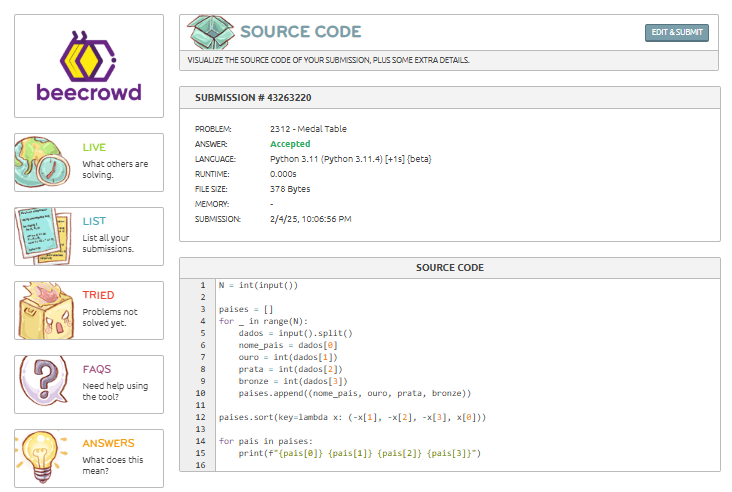
\includegraphics[width=0.7\textwidth]{figuras/questao 2.png}
	}
	\label{fig:questao 2}
\end{figure}

\section{Cálculo da complexidade no tempo do problema 2}


O código \ref{lst:codigo-problema1} começa lendo um inteiro N (número de países). Em seguida, ele lê N linhas, onde cada linha contém o nome do país e a quantidade de medalhas . A leitura de cada linha e o processamento são operações de tempo constante, O(1). O loop que lê os dados do N países tem complexidade O(N), pois o código executa esse processo N vezes através do for.
   
Na linha 12, o código \ref{lst:codigo-problema1} usa o método sort para ordenar a lista paises. O parâmetro key especifica a ordem da ordenação, que é primeiro por ouro , depois por prata, depois por bronze, e finalmente por nome .O algoritmo de ordenação utilizado pelo Python é o Timsort, que tem complexidade O(N log N) no pior caso, onde N é o número de elementos a serem ordenados.
  
Após a ordenação o código imprime os resultados dos países ordenados. A operação de impressão para cada país é O(1) e o loop percorre a lista de países o que resulta em uma complexidade de O(N) para esta parte.

Análise final:
A leitura dos dados tem complexidade O(N), a ordenação tem complexidade O(N log N), que é o passo dominante e a impressão tem complexidade O(N).

Complexidade total:
A operação dominante é a ordenação, que tem complexidade O(N log N).
As outras operações (leitura de dados e impressão) têm complexidades O(N), que são menores em comparação à ordenação.

\begin{lstlisting}[language=Python, caption={Código de implementação do algoritmo de implementação do problema 2}, label={lst:codigo-problema2}]
N = int(input())

paises = []
for _ in range(N):
    dados = input().split()
    nome_pais = dados[0]
    ouro = int(dados[1])
    prata = int(dados[2])
    bronze = int(dados[3])
    paises.append((nome_pais, ouro, prata, bronze))

paises.sort(key=lambda x: (-x[1], -x[2], -x[3], x[0]))

for pais in paises:
    print(f"{pais[0]} {pais[1]} {pais[2]} {pais[3]}")
\end{lstlisting}

\section{Modelagem dinâmica}
\label{sec:modelagemdinamica}
